\section{Results}
\label{sec:results}

\begin{figure*}[ht]
    \centerline{\framebox{
    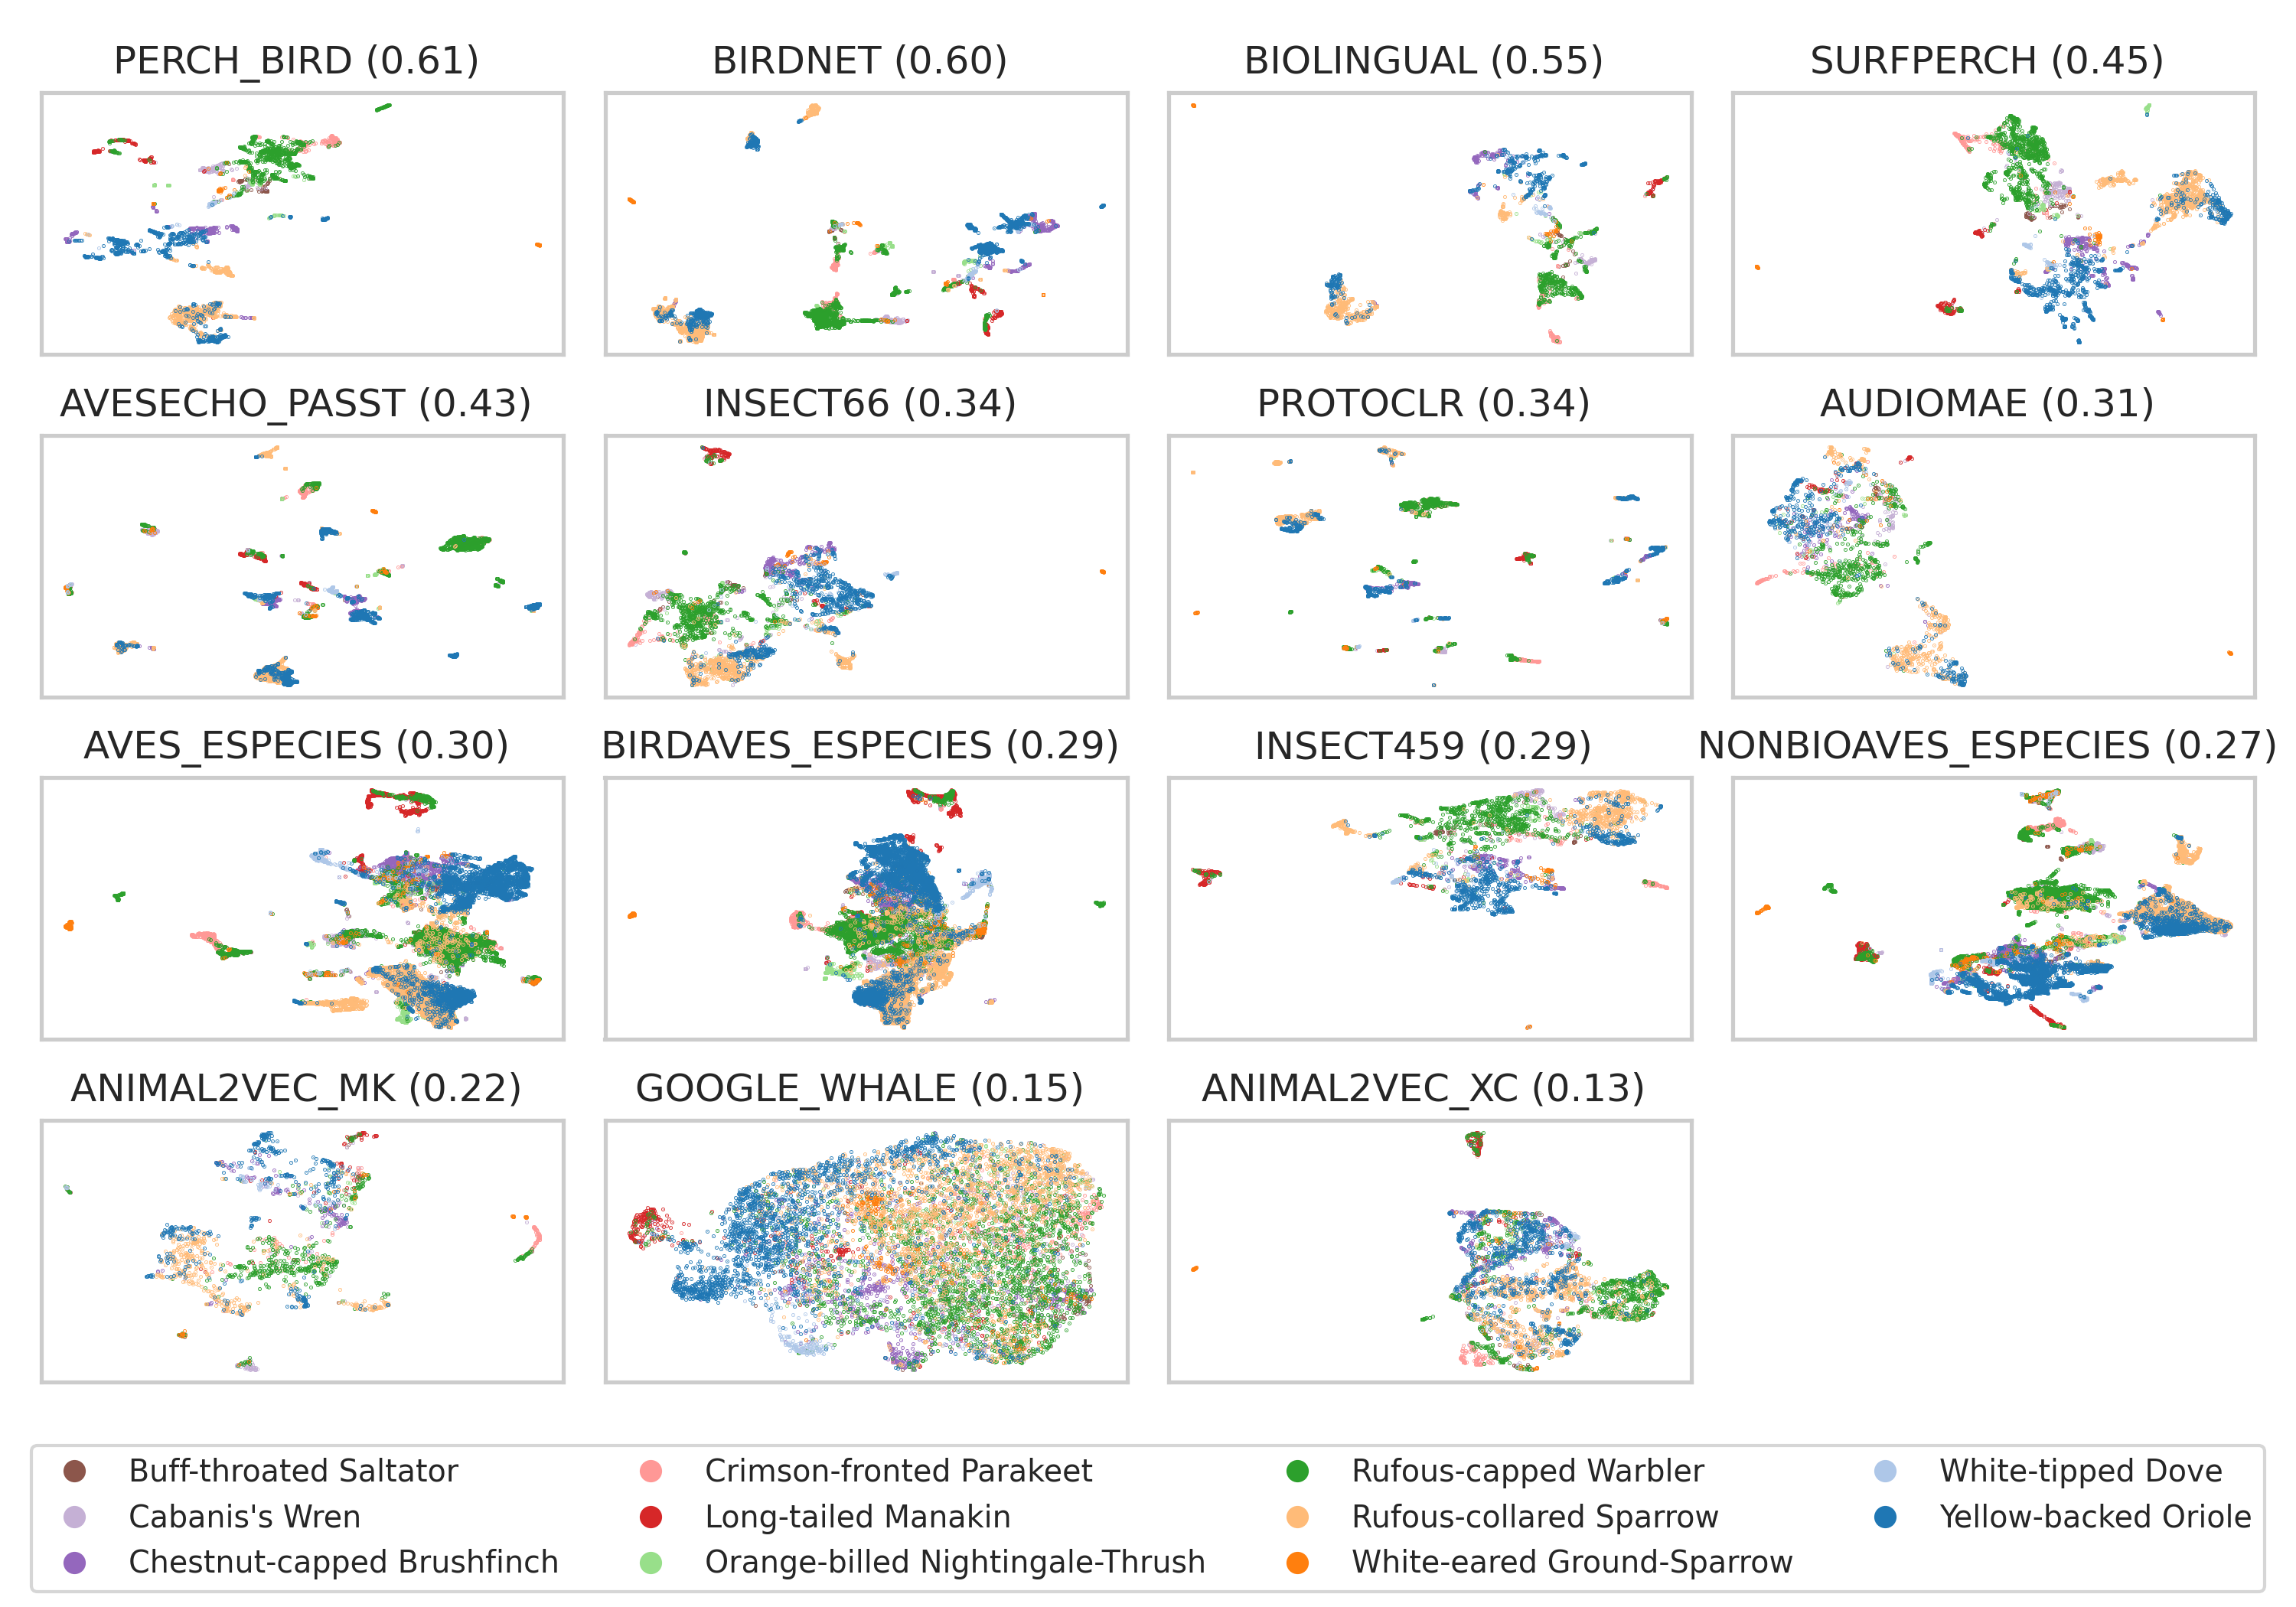
\includegraphics[width=16.3cm]{Sections/imgs/normal_overview.png}}}
    \caption{Two-dimensional embedding spaces of all feature extractors, sorted descending by their clustering performance of AMI values (indicated next to their name) from top left to bottom right.
    Given the different input lengths of the feature extractors, the number of embeddings vary significantly.
    Colors correspond to the class labels, which are 11 different tropical bird species.}
    \label{fig:embeds}
\end{figure*}

% Embeddings spaces of are visualized using UMAP in are generated from the input data using all feature extractors and then the dimensionality reduction algorithm UMAP is used to visualize the data in two dimensions.
% The results are shown in Fig. \ref{fig:embeds}.

Two-dimensional UMAP embeddings are shown in Fig.~\ref{fig:embeds}.
The worst performing feature extractors, produce large unstructured clouds of mixed color, indicating that no significant clustering is achieved.
In the first and second row, feature extractors can be seen to separate the embeddings into meaningful clusters.
It is noticeable that some feature extractors such as AvesEcho\_PaSST and ProtoCLR seem to generate more subclusters than most other feature extractors.
The seven best performing feature extractors are all trained using supervised learning and the top three additionally trained on bird vocalizations.
All three of the AVES models (BirdAVES, AVES and NonBioAVES) reach similar performances in spite of big differences in their fine-tuning datasets \cite{hagiwara_aves_2022}.


\begin{table}[t]
  
  \caption{List of feature extractors compared in this study. }
  \label{tab:results}
  \centering
  \begin{tabular}{|l|ccc|}
    \hline
    \textbf{bird data}& \multicolumn{3}{c|}{classification (macro accuracy)} \\
    \hline
    category &
    original &
    umap &
    pca \\
    \hline
    ssl & 0.617& 0.619& 0.587 \\
    supl & 0.695& 0.711& 0.66 \\
    bird & 0.712& 0.723& 0.607 \\
    non-bird & 0.609& 0.618& 0.658 \\
    \hline
    & \multicolumn{3}{c|}{clustering (AMI)} \\
    \hline
    ssl & 0.256& 0.405& 0.25 \\
    supl & 0.418& 0.476& 0.414 \\
    bird & 0.426& 0.479& 0.411 \\
    non-bird & 0.271& 0.413& 0.276 \\
    \hline
    \textbf{frog data}& \multicolumn{3}{c|}{classification (macro accuracy)} \\
    \hline
    category &
    original &
    umap &
    pca \\
    \hline
    ssl & 0.682& 0.679& 0.601 \\
    supl & 0.668& 0.655& 0.673 \\
    bird & 0.705& 0.698& 0.629 \\
    non-bird & 0.638& 0.627& 0.662 \\
    \hline
    & \multicolumn{3}{c|}{clustering (AMI)} \\
    \hline
    ssl & 0.414& 0.508& 0.418 \\
    supl & 0.488& 0.546& 0.49 \\
    bird & 0.5& 0.558& 0.503 \\
    non-bird & 0.411& 0.5& 0.414 \\
    \hline
  \end{tabular}
\end{table}


% ssl & 0.617& 0.619& 0.587 \\
% supl & 0.695& 0.711& 0.66 \\
% bird & 0.712& 0.723& 0.607 \\
% non-bird & 0.609& 0.618& 0.658 \\
% \\hline
    
% \\hline
% ssl & 0.256& 0.405& 0.25 \\
% supl & 0.418& 0.476& 0.414 \\
% bird & 0.426& 0.479& 0.411 \\
% non-bird & 0.271& 0.413& 0.276 \\
% \\hline
    
% \\hline
% category &
% original &
% umap &
% pca \\
% \\hline
% ssl & 0.682& 0.679& 0.601 \\
% supl & 0.668& 0.655& 0.673 \\
% bird & 0.705& 0.698& 0.629 \\
% non-bird & 0.638& 0.627& 0.662 \\
% \\hline
    
% \\hline
% ssl & 0.414& 0.508& 0.418 \\
% supl & 0.488& 0.546& 0.49 \\
% bird & 0.5& 0.558& 0.503 \\
% non-bird & 0.411& 0.5& 0.414 \\

% \begin{figure}[ht]
%     \centerline{\framebox{
%         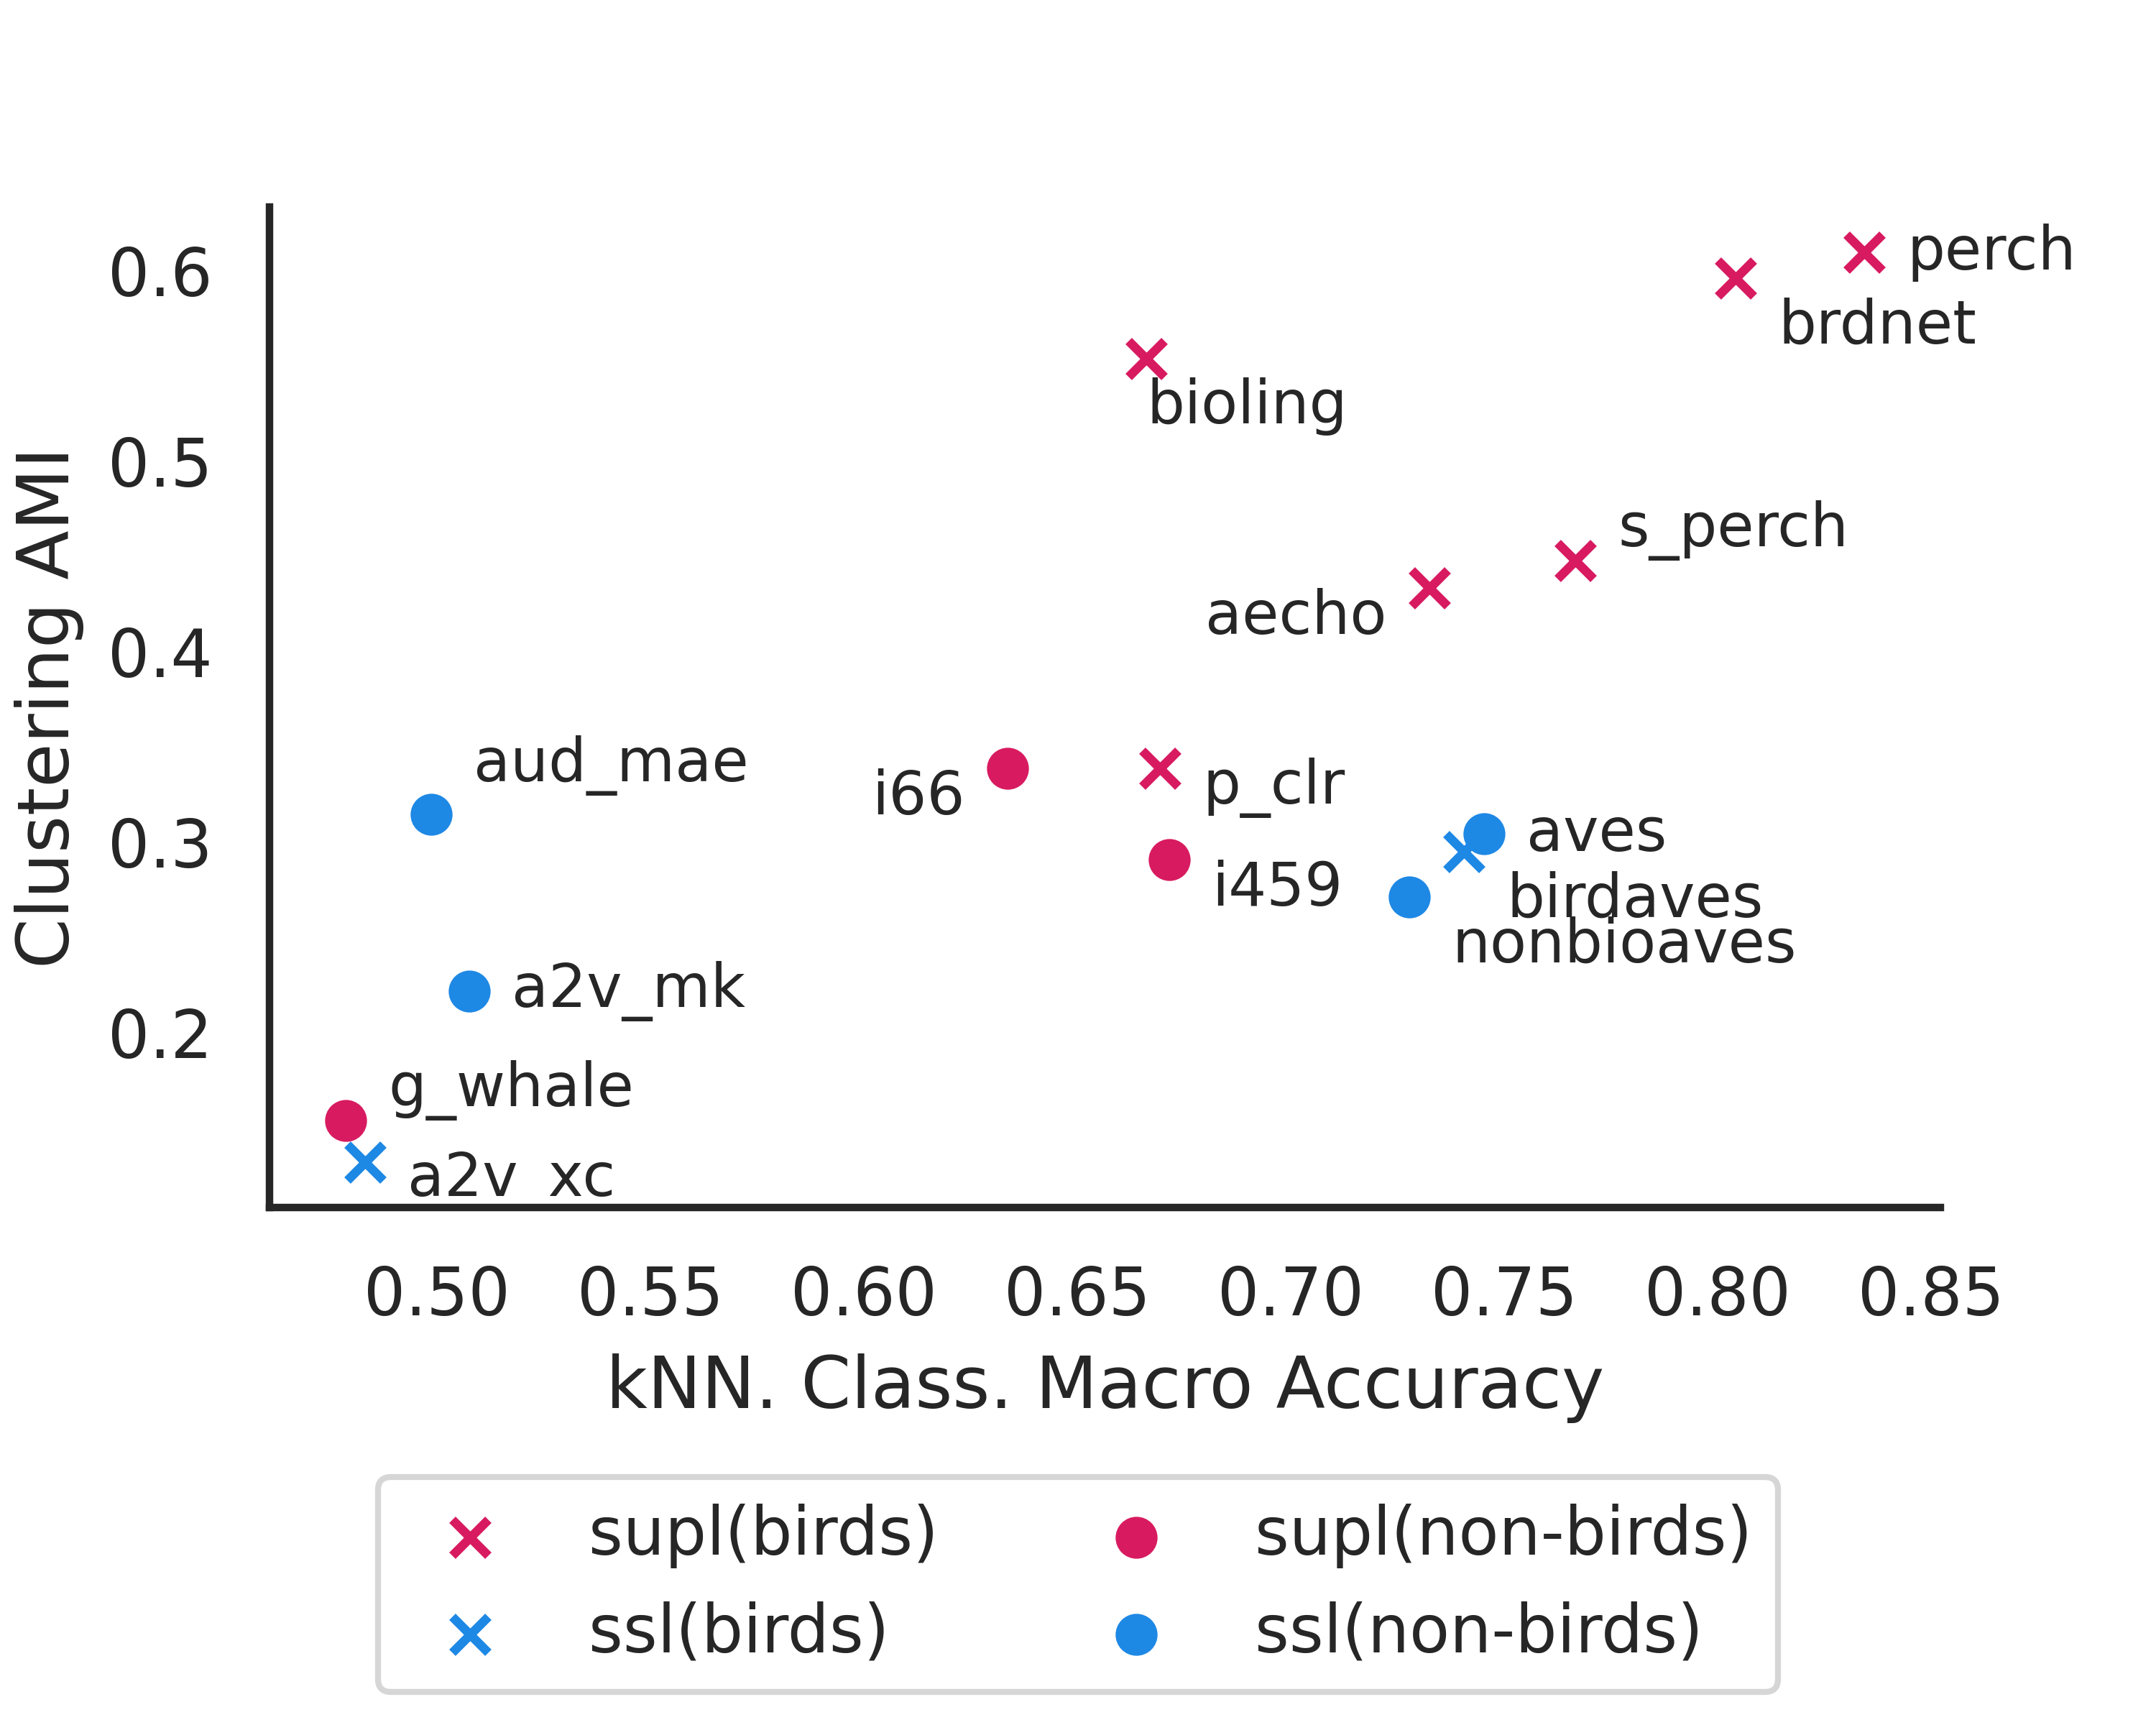
\includegraphics[width=7.8cm]{Sections/imgs/scatterplot_clust_vs_class_nt_knn_normal.png}}}
%         \caption{Comparison of feature extractors by learning paradigm and training data. Abbreviated names correspond to abbrev. column in Tab.~\ref{tab:bacpipe_models}. The x-axis shows clustering results of AMI while the y-axis shows macro accuracy results of kNN classification. Colors correspond to supervised learning and self-supervised learning feature extractors, while symbols separate bird and non-bird training data.}
%         \label{fig:subl_vs_ssl}
%     \end{figure}
    
% To investigate how training setup and training data affect performance, Fig. \ref{fig:subl_vs_ssl} shows a scatterplot of the different feature extractors.
Performance is evaluated by macro accuracy of knn classification on the x-axis and AMI of clustering on the y-axis.
% AMI is chosen to evaluate clustering performance as we are primarily interested to see how well the KMeans clustering agrees with the ground truth.

When focussing on the y-axis, all self-supervised learning feature extractors (in red) reach clustering performances under 0.31.
Performance by kNN classification is more equally distributed, however, again supervised learning feature extractors reach the six highest values.
Furthermore, Animal2vec\_XC, the only self-supervised learning feature extractor that was not fine-tuned, performs poorly by both clustering and kNN classification.
Google\_Whale represents the only supervised learning feature extractor performing very poorly by clustering and kNN classification.

Comparing by training data, feature extractors trained on only or including bird datasets outperform the other feature extractors by kNN classification and even more so by clustering.
Aside from ProtoCLR the supervised learning models that are also trained on birds vastly outperform all other models in the combination of clustering and kNN classification.
Perch and BirdNET lead in both clustering and kNN classification by a large margin.
Animal2vec\_XC is the only two feature extractor trained on birds that performs poorly.
Biolingual, which was trained on large bird databases using a multi-modal approach performs well by clustering, but comparably poorly by kNN classification.

When referring back to Table \ref{tab:bacpipe_models} embedding dimension does not correlate with clustering or kNN classification performance.
Furthermore, the only two feature extractors trained on marine sounds, Google\_Whale and SurfPerch (trained on birds and marine sounds) reach very different performances.
    
\begin{figure}[ht]
    \centerline{\framebox{
    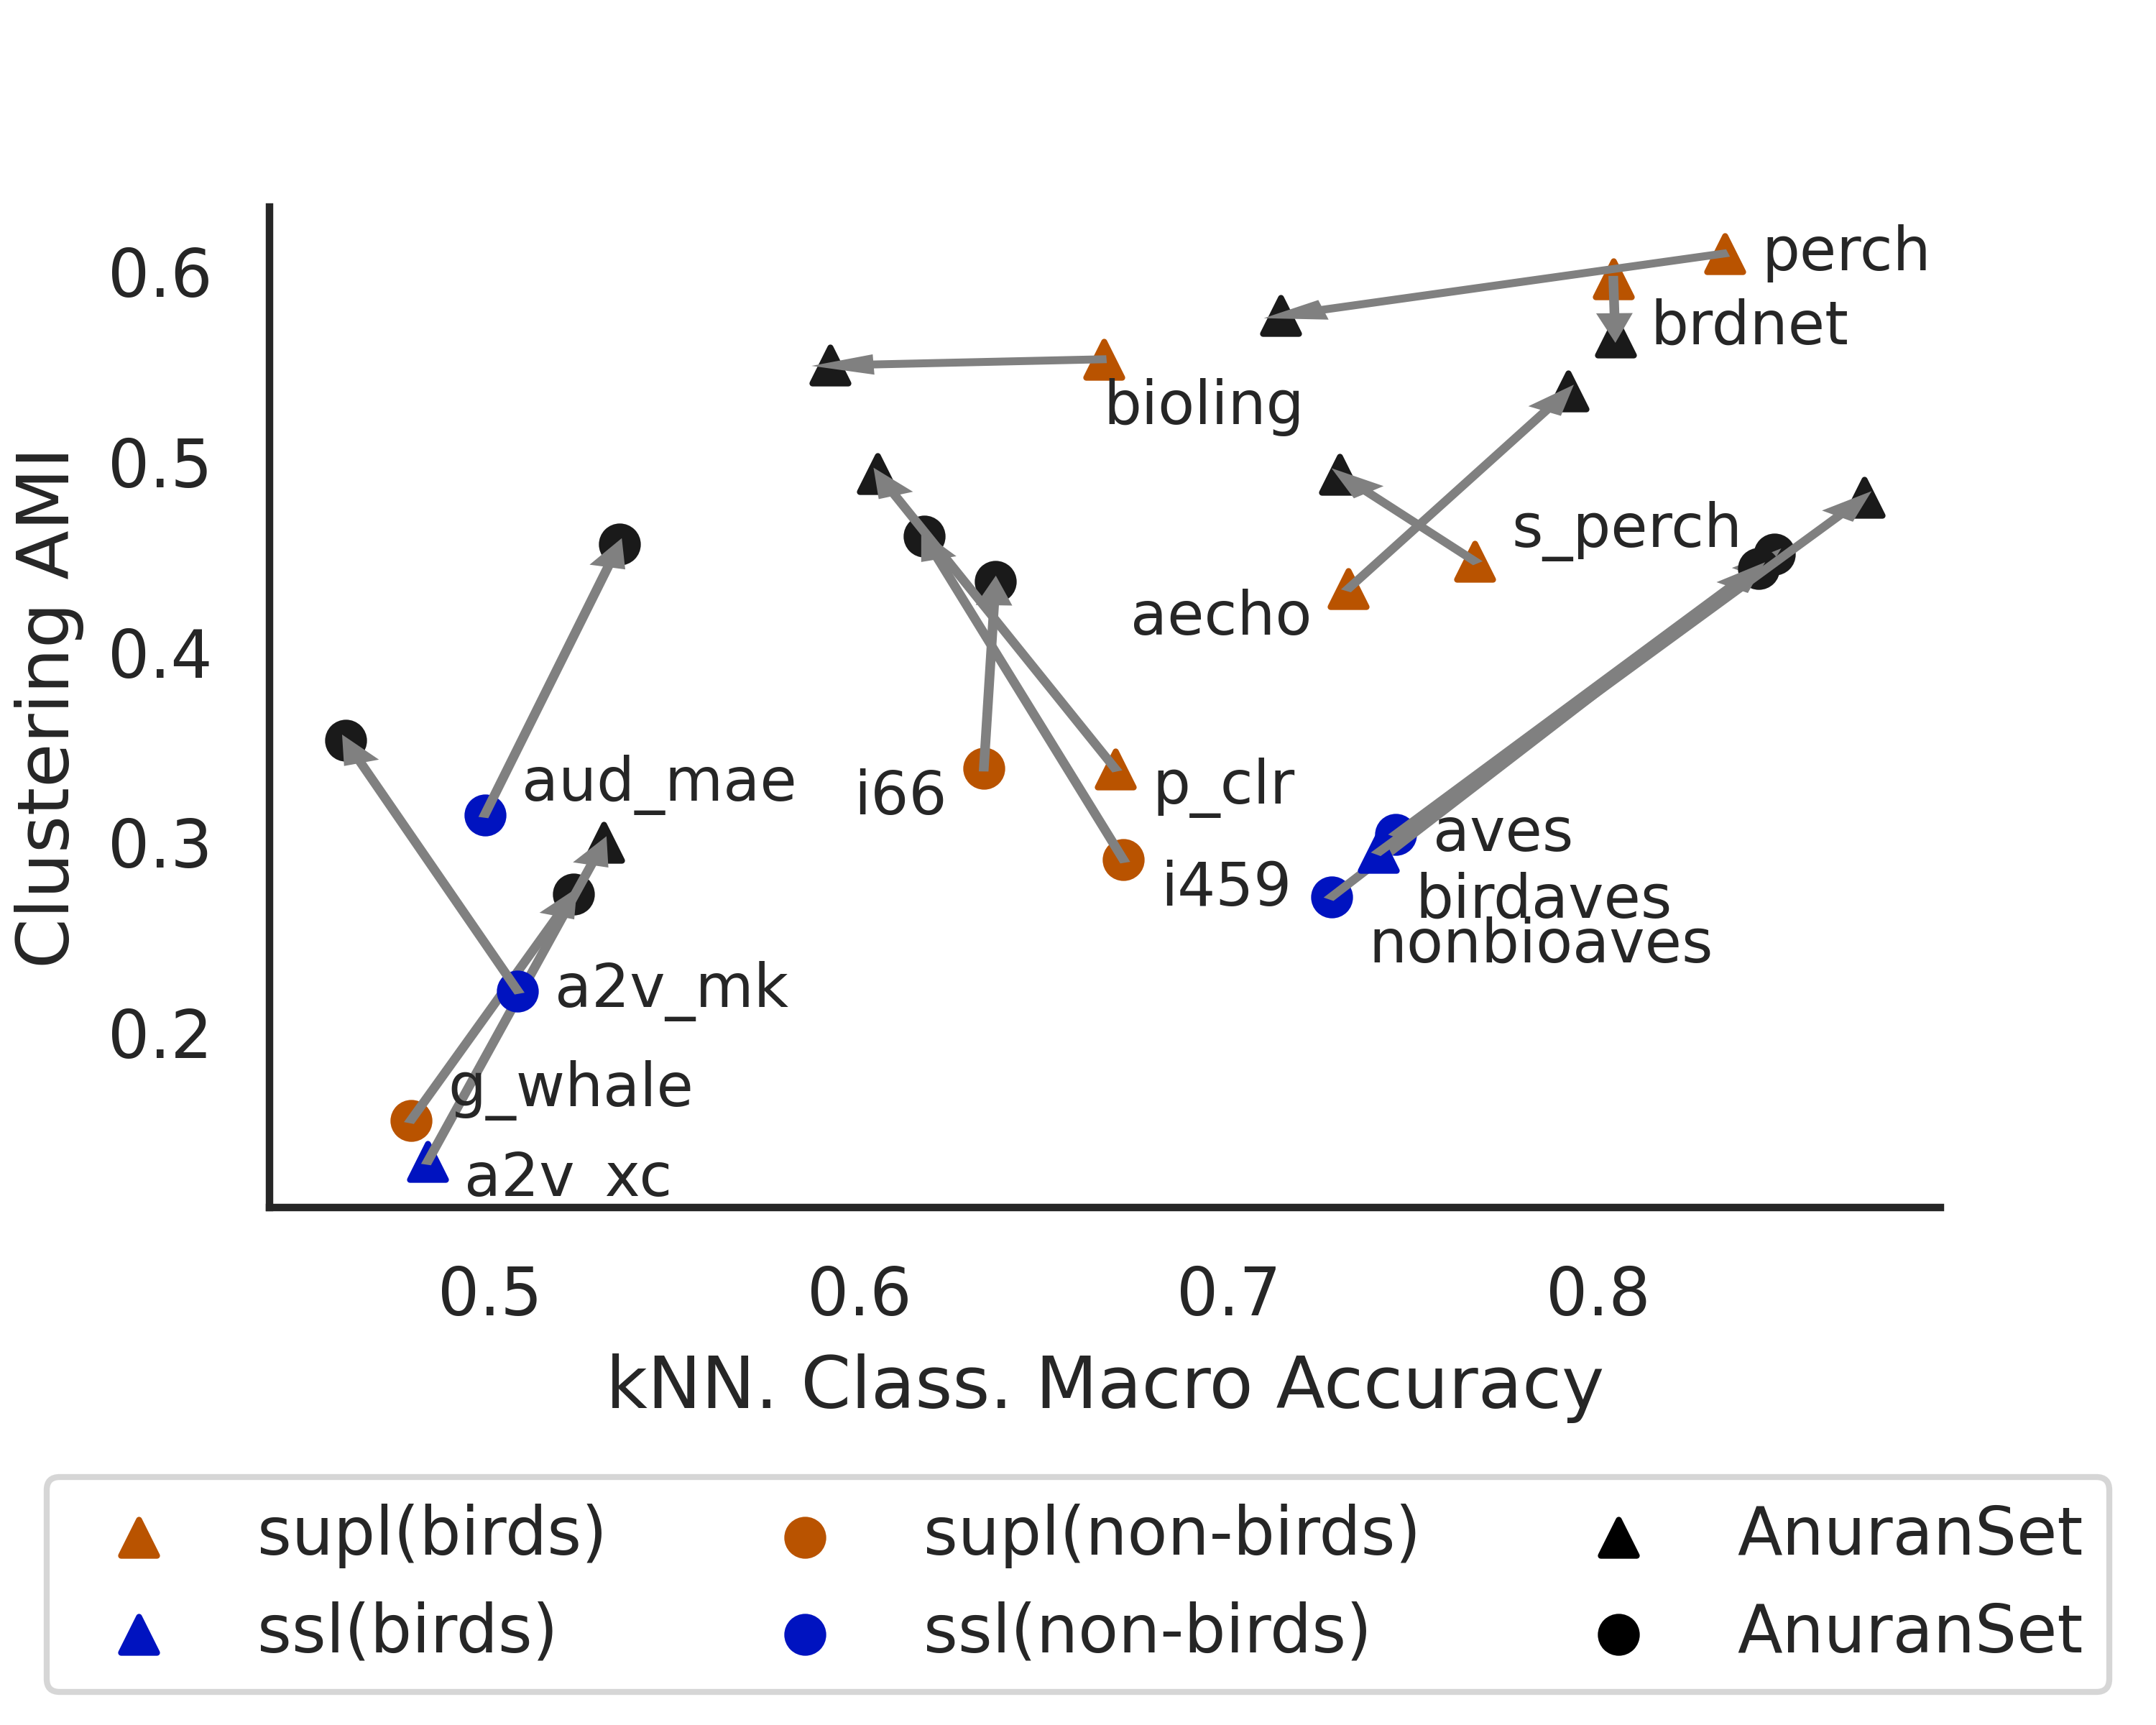
\includegraphics[width=7.8cm]{Sections/imgs/scatterplot_clust_vs_class_neotrop_anuran_normal.png}}}
    \caption{Comparison of feature extractor performance for bird and frog datasets. 
    Axes, symbols and colors points correspond to the same as in Fig. \ref{fig:subl_vs_ssl}.
    Here, black points show the performance of each feature extractor on the bird dataset.
    Red and blue points show the performance on the frog dataset. 
    The grey arrow shows the performance change from the bird to the frog dataset.}
    \label{fig:orig_vs_ump}
\end{figure}

To highlight performance changes once the feature extractors are applied to a dataset different from their training domain, Fig. \ref{fig:orig_vs_ump} shows the performance on the bird dataset (black) and the frog dataset (red and blue) connected by an arrow.
Aside from Perch, BirdNET and Biolingual all feature extractors increase in clustering performance when applied to the frog dataset.
All self-supervised feature extractors improve in clustering performance and aside from Animal2vec\_MK also in kNN classification.
The self-supervised AVES feature extractors (BirdAVES, AVES and NonBioAVES) drastically improve in both clustering and kNN classification on the frog dataset.
So much so, that all three outperform all other feature extractors by kNN classification.
Among supervised learning feature extractors, kNN classification performance changes are more varied.
All non-bird trained feature extractors improve in clustering.
From the supervised bird trained feature extractors, only AvesEcho improves in both clustering and kNN classification.
Again, all bird trained feature extractors except for Animal2vec\_XC outperform the rest by clustering on the frog dataset.
The top 6 models by clustering are again the supervised learning bird trained feature extractors.
However, by kNN classification, results are more mixed by both training paradigm and training domain.
